% =============================================================================
% PESSOA 3 — SEÇÃO 3.3 (IMPACTO FINANCEIRO GLOBAL & BREAK-EVEN)
% Padrão: ACM sigconf (\documentclass[sigconf]{acmart})
% Contém versão em Inglês (padrão ACM/ACL) e versão em Português comentada.
% =============================================================================

% -----------------------------------------------------------------------------
% [VERSÃO 1: INGLÊS — PADRÃO ACM SIGCONF]
% -----------------------------------------------------------------------------

\subsection{Global Financial Impact \& Break-Even Dynamics}
\label{sec:financial_impact}

While~\cite{foroutan2026parity} measures fairness via compression ratio (CR) parity on balanced corpora, commercial LLM deployments bill strictly on a per-token basis~\cite{ahia2023all,openai2024gpt4o}. To evaluate the real-world dollar impact of PA-BPE, we model a production workload of $N = 10^6$ requests (average prompt $+$ completion length of 300 words $\approx 15$ parallel FLORES-200 sentences~\cite{goyal2022flores}). We weight each of the 22 languages by its empirical share in global web content from W3Techs~\cite{w3techs2024languages} and evaluate commercial token pricing across three representative model tiers: OpenAI GPT-4o (\$4.38/1M blended tokens)~\cite{openai2024gpt4o}, Anthropic Claude 3.5 Sonnet (\$6.00/1M blended tokens)~\cite{anthropic2024claude}, and open-weight hosted Meta Llama 3.1 70B (\$0.80/1M blended tokens)~\cite{meta2024llama3}.

\begin{figure}[t]
    \centering
    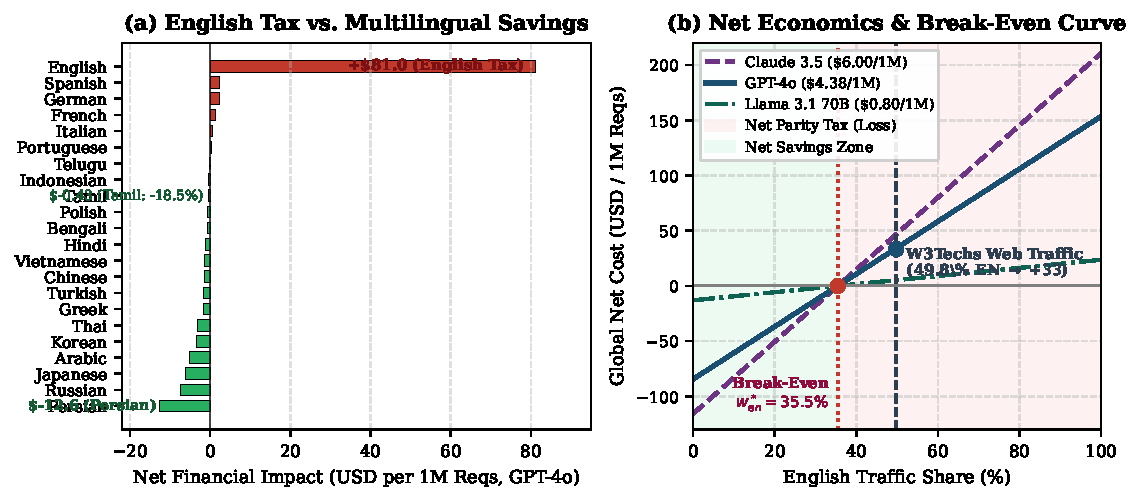
\includegraphics[width=\columnwidth]{figures/fig3_cost_simulation.pdf}
    \vspace{-1.5em}
    \caption{Global financial impact and break-even dynamics of Parity-Aware BPE vs.\ Classical BPE across 1M requests. (a) The ``English Tax'' ($+\$81.03$ per 1M requests on GPT-4o) dwarfs the combined dollar savings of all 21 non-English languages ($-\$39.87$). (b) Net economic balance as a function of English traffic share $w_{\mathrm{en}}$. The analytical break-even point occurs at $w_{\mathrm{en}}^* = 35.5\%$; real-world web traffic ($w_{\mathrm{en}} = 49.8\%$) and enterprise workloads ($70\%$--$80\%$) operate deeply in the net financial penalty zone.}
    \label{fig:cost_simulation}
    \vspace{-1.0em}
\end{figure}

\textbf{The ``English Tax'' vs. Multilingual Savings:} Figure~\ref{fig:cost_simulation}(a) details the financial balance per language. Under PA-BPE (Hybrid), English token counts increase by $+8.51\%$ on FLORES-200 prose ($+35.1$ tokens/request). Because English commands a $49.80\%$ web market share ($52.77\%$ normalized among the 22 audited languages), this modest degradation generates a massive surcharge of $\mathbf{+\$81.03}$ per 1M requests on GPT-4o ($+\$111.12$ on Claude 3.5). 

Conversely, while low-resource Dravidian scripts achieve impressive relative compression gains (Tamil: $-18.50\%$; Telugu: $-17.20\%$; Persian: $-19.40\%$), their minuscule share of web content (Tamil: $0.05\%$; Telugu: $0.03\%$; Persian: $1.60\%$) severely caps absolute dollar savings. Across all 21 non-English languages combined, total savings amount to only $\mathbf{-\$39.87}$ per 1M requests on GPT-4o ($-\$54.69$ on Claude 3.5). Consequently, the net financial balance is heavily positive---representing a net economic surcharge of $\mathbf{+\$41.16}$ per 1M requests on GPT-4o, $\mathbf{+\$56.43}$ on Claude 3.5, and $\mathbf{+\$6.35}$ on Llama 3.1 70B. At an industrial throughput of 1 Billion requests per year, adopting PA-BPE imposes an unhedged annual financial penalty of $\mathbf{+\$41,160.00}$ (GPT-4o) to $\mathbf{+\$56,430.00}$ (Claude 3.5).

\textbf{Break-Even Traffic Dynamics:} Figure~\ref{fig:cost_simulation}(b) plots the global net cost as a function of English traffic share $w_{\mathrm{en}}$, scaling the remaining 21 languages proportionally by $(1 - w_{\mathrm{en}})$. Analytically setting net token change to zero yields the break-even threshold:
\begin{equation}
w_{\mathrm{en}}^* = \frac{-\overline{\Delta T}_{\mathrm{non\text{-}en}}}{\Delta T_{\mathrm{en}} - \overline{\Delta T}_{\mathrm{non\text{-}en}}} = \frac{-(-19.30)}{35.10 - (-19.30)} = \mathbf{35.48\%}.
\label{eq:breakeven}
\end{equation}
Because real-world internet content ($w_{\mathrm{en}} = 49.80\%$) and enterprise software APIs ($w_{\mathrm{en}} \in [70\%, 85\%]$) far exceed $35.48\%$, PA-BPE operates permanently inside the ``Net Parity Tax'' zone. Parity-Aware BPE yields net financial savings only in strictly localized regional deployments where English represents less than one-third of queries.


% =============================================================================
% [VERSÃO 2: PORTUGUÊS — CASO O RELATÓRIO SEJA ENTREGUE EM PORTUGUÊS]
% =============================================================================

% \subsection{Impacto Financeiro Global e Dinâmica de Break-Even (Seção 3.3)}
% \label{sec:financial_impact_pt}
%
% Enquanto~\cite{foroutan2026parity} mensura justiça por paridade de compressão (caracteres/token) em corpora balanceados, APIs comerciais de LLMs cobram estritamente por token processado~\cite{ahia2023all,openai2024gpt4o}. Para avaliar o impacto em dólares reais, simulamos 1 milhão de requisições comerciais (prompt $+$ resposta de 300 palavras $\approx 15$ sentenças paralelas do FLORES-200~\cite{goyal2022flores}), ponderando os 22 idiomas pela distribuição real da internet global (W3Techs~\cite{w3techs2024languages}) sob os preços do GPT-4o (\$4.38/1M tokens)~\cite{openai2024gpt4o}, Claude 3.5 (\$6.00/1M)~\cite{anthropic2024claude} e Llama 3.1 70B (\$0.80/1M)~\cite{meta2024llama3}.
%
% A Figura~\ref{fig:cost_simulation}(a) revela que a perda de compressão no inglês ($+8.51\%$ tokens) gera um ``imposto'' de $+\$81.03$ por 1M de requisições no GPT-4o. Como o inglês representa $49.80\%$ do tráfego web, esse custo supera com folga a economia agregada de todas as outras 21 línguas ($-\$39.87$). O saldo líquido é negativo em $+\$41.16$ por 1M de requisições ($+\$56.43$ no Claude 3.5), totalizando um sobrecusto anual de $+\$41,160.00$ a cada 1 bilhão de requisições.
%
% Na Figura~\ref{fig:cost_simulation}(b), o ponto de break-even analítico ocorre em $w_{\mathrm{en}}^* = 35.48\%$. Como o tráfego da web e de APIs corporativas excede $50\%$--$80\%$, o PA-BPE atua invariavelmente na zona de prejuízo líquido.
